\chapter{Fusilli: Developing a Data Fusion Python Library}
\label{fusilli_development}

The previous chapter explored multimodal data in a relatively simple setting of a survival analysis model.
In the field of machine learning, multimodal data can be integrated as it was in the Cox model, by concatenating the data before inputting into the model, or by using more complex methods that aim to capture the potentially non-linear relationships between the modalities.
These techniques fall under the umbrella of multimodal data fusion.

This chapter discusses multimodal data fusion in more detail and describes the development of Fusilli, a Python package for multimodal data fusion experimentation and analysis.

\section{Introduction}

Multimodal data fusion is the process of combining data from different sources to make predictions or decisions, often through the use of deep learning.
The goal of combining different modalities is to improve the performance of a model by leveraging the relevant information from each modality and fusing them in a way that improves the model's performance.
There are many research fields where multimodal data fusion is used, such as in agriculture to predict crop yields and detect diseases~\cite{s.s.gopiMultimodalMachineLearning2023, patilRiceFusionMultimodalityData2022}, in disaster management to analyse response scenarios from audio and social media posts~\cite{algiriyageMultisourceMultimodalData2021}, and in robotics to help direct the robots with multiple sensors~\cite{duanMultimodalSensorsMLBased2022}.
Moreover, the types of models used in multimodal data fusion can vary widely, from geometric deep learning to relatively simple neural network architectures~\cite{cuiDeepMultimodalFusion2022}.

%In the context of my PhD, I am investigating multimodal data fusion for MND prognosis prediction.
%There has been minimal research on deep learning for prognosis prediction in MND~\cite{pancottiDeepLearningMethods2022, mullerExplainableModelsDisease2021}, and only one model created for deep-learning based multimodal data fusion~\cite{vanderburghDeepLearningPredictions2017}.
%However, there are many data fusion models that have been used in other fields that could be directly applicable to MND .
%There have been systematic reviews on the topic of data fusion that compare models, but only qualitatively~\cite{cuiDeepMultimodalFusion2022, gaoSurveyDeepLearning2020, stahlschmidtMultimodalDeepLearning2022, yanDeepMultiviewLearning2021}.
%Therefore, with limited knowledge from literature on the best models for MND data, it is important to experiment with a wide variety of models to find the best one for the task.

My PhD investigates multimodal data fusion for predicting MND prognosis, an area with minimal deep learning research~\cite{pancottiDeepLearningMethods2022, mullerExplainableModelsDisease2021} and only one model specially-created for deep-learning based multimodal data fusion~\cite{vanderburghDeepLearningPredictions2017}.
Despite systematic reviews on the topic attempting qualitative comparison between models in many areas of applications~\cite{cuiDeepMultimodalFusion2022, gaoSurveyDeepLearning2020, stahlschmidtMultimodalDeepLearning2022, yanDeepMultiviewLearning2021}, a lack of quantitative comparison necessitates experimentation with many models from other fields to identify the most effective for MND prognosis prediction.

%Obtaining this wide variety of models to experiment with, however, is not a straightforward process for a number of reasons.
%Firstly, the terminology used to describe what I have chosen to call ''multimodal data fusion'' varies widely, with terms such as but not limited to multi-view, cross-heterogeneous, multi-source, and integrated learning.
%Secondly, the studies that introduce these models often do not include code for the reader to run the model.
%Morever, when code is included, it is often written in different languages, with varying guidance, quality, and maintenance.
Acquring a diverse range of models for experimentation is made difficult by the use of inconsistent terminology and the common unavailability of maintained, quality code provided alongside studies.

A way to address these problems is to create a curated collection of models for somebody interested in multimodal data fusion to consult.
As far as I am aware, there are three Python packages that house collections of deep learning based data fusion models: ''Multi-view-AE''~\cite{aguilaMultiviewAEPythonPackage2023}, ''CCA-Zoo''~\cite{chapmanCCAZooCollectionRegularized2021}, and ''pytorch-widedeep''~\cite{zaurinPytorchwidedeepFlexiblePackage2023}.
However, each of these packages only includes models with specific frameworks (autoencoders, CCA, and Google's ''wide and deep'' models, respectively), which limits the variety of models available for comparison.

Therefore, I aimed to develop a Python package for training and comparing multimodal data fusion models with any architecture.
This Python package is named Fusilli, as a portmanteau of ''fuse easily''.
Fusilli works by taking the user's multimodal data and training it on a variety of models, and then comparing the models' performances.

\section{Development and Implementation}

\subsection{Software Design Choices}

Before developing Fusilli, the following design goals were set to ensure the package would be useful for a wide range of users and tasks, as well as for my own research.
\vspace{0.3cm}

\noindent\textbf{Modularity}: Fusilli should be modular, meaning that the various functionalities within the package should be independent of each other.
This would allow for easy addition of new models in the future and easy adjustments to the package's functionality.
Testing, which is the process of writing code to check that the package works as expected, would also be easier with a modular design, and so the package would be more reliable.

\vspace{0.3cm}

\noindent\textbf{Beginner-friendly and expert-friendly}:  Fusilli should be beginner-friendly, with users able to compare the different models without needing expertise in deep learning or Python programming.
This would make it different from other similar packages, which require the user to set up their own experiments.

On the other hand, Fusilli should also be expert-friendly, with users who are more capable being able to change the training parameters, modify the models, and access the trained models for further experiments.

\vspace{0.3cm}

\noindent\textbf{Wide applicability}:
Fusilli should include a wide variety of models, to ensure that the best model for a given task can be found.
Moreover, this would ensure that the package is useful for a wide range of users, as different users may have different requirements for model architectures based on their task and data.

\vspace{0.3cm}

\noindent\textbf{Support for two modalities}: The models in Fusilli will support data fusion between either two types of tabular data (e.g. clinical data and brain region volumes data) or between an image and tabular data (e.g. MRI images and clinical data).
For wide applicability, Fusilli should be able to handle two-dimensional and three-dimensional images, and tabular data of any size.

\vspace{0.3cm}

\noindent\textbf{Support for different prediction tasks}: The prediction tasks that Fusilli should support are regression and classification.
From the literature, these are the most common tasks for multimodal data fusion, and are the tasks that I am interested in for my own research.


\subsection{Implementation}

Fusilli was implemented in Python, using the PyTorch and PyTorch Lightning libraries for deep learning.
PyTorch is a popular library for deep learning, and is known for its flexibility and ease of use.

\noindent For a user to apply Fusilli to their own problem, they must specify:
\begin{itemize}
  \setlength\itemsep{-0.5em}
    \item \textbf{Data}: The user's data, which must be in the form of a .csv file for tabular data, and .pt files for images.
    \item \textbf{Task}: The task that the user wants to perform, which can be either regression or classification (binary or multiclass).
    \item \textbf{Models}: The models that the user wants to compare, which can be any of the models included in Fusilli.
    \item \textbf{Output}: The output directory for the trained models and the results of the experiments.
\end{itemize}

\noindent The user can also specify experiment specifics, which are set to default values if not specified.
Examples of experiment specifics include the training and validation data splits, the maximum number of epochs to train for, and the batch size.
The user can also modify model hyperparameters and architectures.

After the user has specified these, the user calls two functions in Fusilli to train the models:
\begin{itemize}
\setlength\itemsep{-0.5em}
    \item \texttt{prepare\_fusion\_data()}: This function prepares the data for training, including splitting it into training and validation sets and running any model-specific data preparation steps.
    \item \texttt{train\_and\_save\_models()}: This function trains the models on the user's data, and outputs the trained models.
\end{itemize}

Finally, the user can call functions to evaluate a single model or compare the models, which will output the performance of the models on the user's validation data or external test data.
The evaluation figures are saved in the output directory, and the user can also access the trained models for further analysis.

\subsection{Fusion Methods}

A literature search was conducted to find models that could be included in Fusilli.
The search criteria aimed to return papers that mentioned machine learning, multimodality, and image and tabular data, with variants of these terms used to capture a wide range of papers.
The resulting papers were checked for relevance and papers were discarded which use the same model as another paper, which happened frequently.

The models were categorised based on the taxonomy defined by Cui and colleagues in their review on data fusion methods for diagnosis and prognosis~\cite{cuiDeepMultimodalFusion2022}.
Figure~\ref{fig:fusilli_taxonomy} is a diagram taken from the review, which shows the general architecture differences between the categories, and Table~\ref{tab:fusilli_taxonomy} includes descriptions of the categories.

\begin{table}
    \centering
    \caption{Descriptions of data fusion model categories used in Fusilli, first proposed by Cui and colleagues~\cite{cuiDeepMultimodalFusion2022}.}
    \label{tab:fusilli_taxonomy}
    \begin{tabular}{|p{0.25\textwidth}p{0.7\textwidth}|}
        \hline
        \textbf{Category} & \textbf{Description} \\ \hline
        \textbf{Operation-based} & Models that fuse data based on operations such as concatenation, addition, or multiplication. This can be done at any point in the model, such as at the input, hidden layers, or output. \\ \hline
        \textbf{Attention-based} & Models that use attention mechanisms to weight the importance of different modalities. \\ \hline
        \textbf{Graph-based} & Models with a graph structure, such as graph convolutional networks, which capture the relationships between the data by treating them as nodes in a graph with edges connecting them representing the relationships. \\ \hline
        \textbf{Subspace-based} & Models that project the data into a joint lower-dimensional space, for example with deep learning methods such as autoencoders. \\ \hline
        \textbf{Tensor-based} & Models that use tensor operations to fuse the data to capture inter- and intra-modality correlations. \\ \hline
    \end{tabular}
\end{table}

%\begin{itemize}
%\setlength\itemsep{-0.5em}
%    \item \textbf{Operation-based}: Models that fuse data based on operations such as concatenation, addition, or multiplication.
%    This can be done at any point in the model, such as at the input, hidden layers, or output.
%    \item \textbf{Attention-based}: Models that use attention mechanisms to weight the importance of different modalities.
%    \item \textbf{Graph-based}: Models with a graph structure, such as graph convolutional networks.
%    \item \textbf{Subspace-based}: Models that project the data into a joint lower-dimensional space, possibly with deep learning methods such as autoencoders.
%    \item \textbf{Tensor-based}: Models that use tensor operations to fuse the data to capture inter- and intra-modality correlations.
%\end{itemize}

\begin{figure}
    \centering
    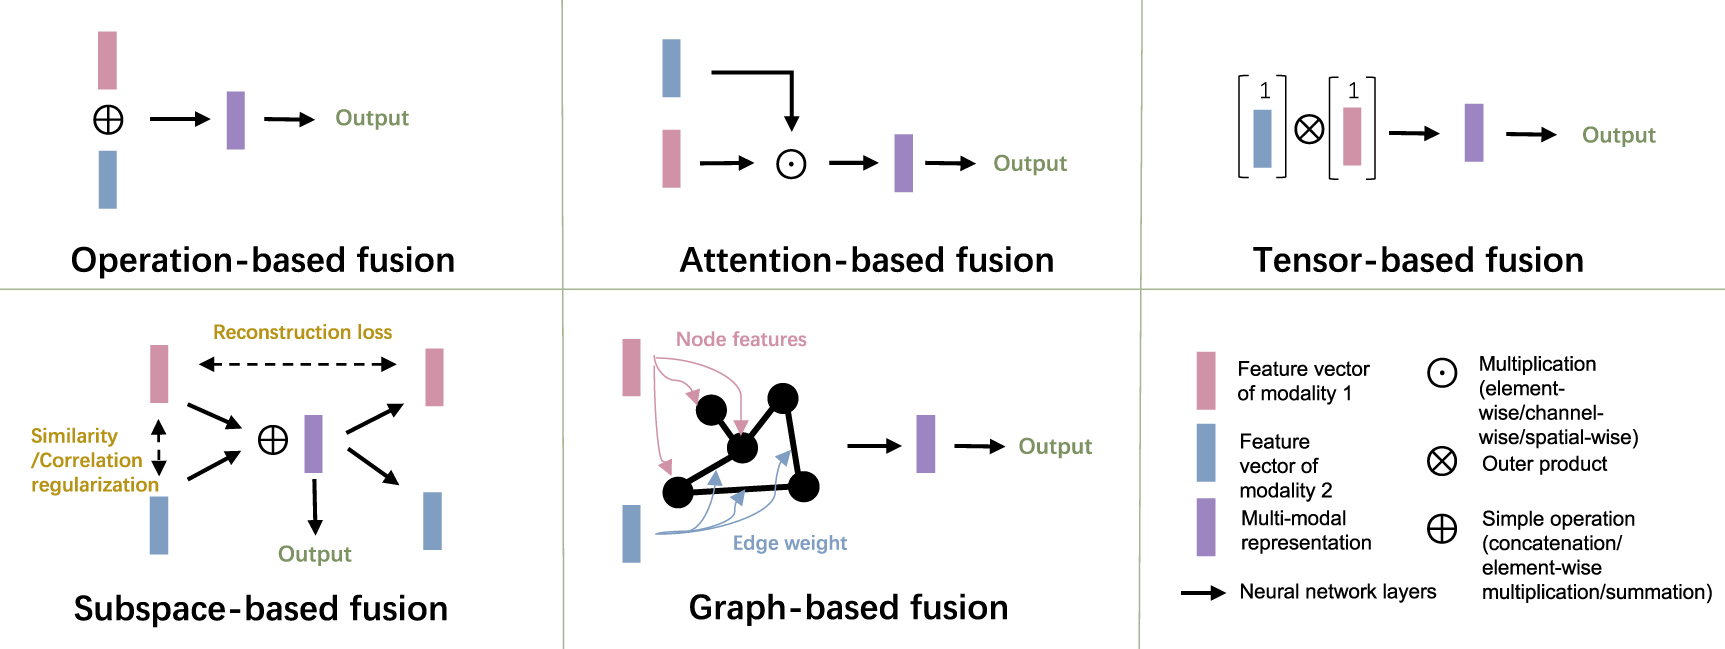
\includegraphics[width=\textwidth]{figures/cui_diagram}
    \caption{Cui and colleagues' diagram of the architecture-based taxonomy of multimodal data fusion models used in Fusilli~\cite{cuiDeepMultimodalFusion2022}.}
    \label{fig:fusilli_taxonomy}
\end{figure}

%Figure~\ref{fig:fusilli_taxonomy} shows the architecture-based taxonomy of multimodal data fusion models, taken from Cui et al.~\cite{cuiDeepMultimodalFusion2022}.

Another common categorisation is ''early'', ''intermediate'', and ''late'' fusion, which refers to the point in the model where the data is fused.
However, this categorisation is too simplistic for the variety of models architectures in Fusilli, and so the architecture-based taxonomy was chosen.

More models were found in the literature than were included in Fusilli due to the time constraints of the project, but the models included in Fusilli were chosen based on their popularity, availability of code, and the variety of architectures they represent.
Moreover, unimodal benchmarks were included in Fusilli to allow for comparison between the multimodal models and unimodal models.

\begin{table}[!ht]
    \caption{A list of the models included in Fusilli v1.2.3, categorised by their fusion method and modalities.
    References are included where applicable, although the Fusilli implementation is not a direct copy of the referenced model, and may have been modified to fit the package's requirements.
    \textbf{Acronyms}: GNN = Graph Neural Network, MCVAE = Multi-Channel Variational Autoencoder.}
    \label{}
    \centering
    \begin{tabular}{|p{8cm}ll|}
        \hline
        \textbf{Model name (and reference where applicable)} & \textbf{Fusion} & \textbf{Modalities} \\ \hline
        Tabular1 uni-modal & Unimodal & Tabular Only \\ \hline
        Tabular2 uni-modal & Unimodal & Tabular Only \\ \hline
        Image unimodal & Unimodal & Image Only \\ \hline
        Activation function map fusion~\cite{chenMDFNetApplicationMultimodal2023} & Operation & Tabular-tabular \\ \hline
        Activation function and tabular self-attention~\cite{chenMDFNetApplicationMultimodal2023} & Operation & Tabular-tabular \\ \hline
        Concatenating tabular data & Operation & Tabular-tabular \\ \hline 
        Concatenating tabular feature maps~\cite{gaoReducingUncertaintyCancer2022} & Operation & Tabular-tabular \\ \hline
        Tabular decision & Operation & Tabular-tabular \\ \hline 
        Channel-wise multiplication net (tabular)~\cite{duanmuPredictionPathologicalComplete2020}  & Attention & Tabular-tabular \\ \hline
        Tabular Crossmodal multi-head attention~\cite{golovanevskyMultimodalAttentionbasedDeep2022}  & Attention & Tabular-tabular \\ \hline
        Attention-weighted GNN~\cite{bintsiMultimodalBrainAge2023} & Graph & Tabular-tabular \\ \hline
        Edge Correlation GNN & Graph & Tabular-tabular \\ \hline 
        MCVAE Tabular~\cite{antelmiSparseMultiChannelVariational2019}  & Subspace & Tabular-tabular \\ \hline
        Concatenating tabular data with image feature maps~\cite{liFusingMetadataDermoscopy2020}  & Operation & Tabular-image \\ \hline
        Concatenating tabular and image feature maps~\cite{gaoReducingUncertaintyCancer2022} & Operation & Tabular-image \\ \hline
        Image decision fusion & Operation & Tabular-image \\ \hline 
        Channel-wise Image attention~\cite{duanmuPredictionPathologicalComplete2020} & Attention & Tabular-image \\ \hline
        Crossmodal multi-head attention~\cite{golovanevskyMultimodalAttentionbasedDeep2022} & Attention & Tabular-image \\ \hline
        Trained Together Latent Image + Tabular Data~\cite{zhaoMultimodalDeepLearning2022} & Subspace & Tabular-image \\ \hline
        Pretrained Latent Image + Tabular Data~\cite{zhaoMultimodalDeepLearning2022} & Subspace & Tabular-image \\ \hline
        Denoising tabular autoencoder with image maps~\cite{yanRicherFusionNetwork2021} & Subspace & Tabular-image \\ \hline
    \end{tabular}
\end{table}

\section{Results}

Fusilli version 1.0.0 was published on 30th November 2023, and has since been updated to version 1.2.3~\cite{townendFlorencejtFusilliFusilli2024}.
Currently, Fusilli is under review for publication in the Journal of Open Source Software (JOSS).
The package has been well-received on GitHub, having been favourited by 142 users and specially cloned by 12 users for their own modifications.
Moreover, I wrote an article on Medium about Fusilli, which has been read by 257 people, and two articles have been written about Fusilli by other people.

Fusilli is documented using Sphinx, a Python documentation generator.
Figure~\ref{fig:fusillidocs} shows an overview of the documentation, which includes tutorials for getting started, guidance for more advanced users, example Python scripts which run the models on simple data, a guide for people to contribute their own models, and the source code documentations.
The page ''Fusion Model Explanations'', partly shown in Figure~\ref{fig:fusillidocs}B, has a diagram and a text explanation for each model in Fusilli, which is useful for users to understand and compare the models' architectures with a standardised diagram style.

\begin{figure}
    \centering
    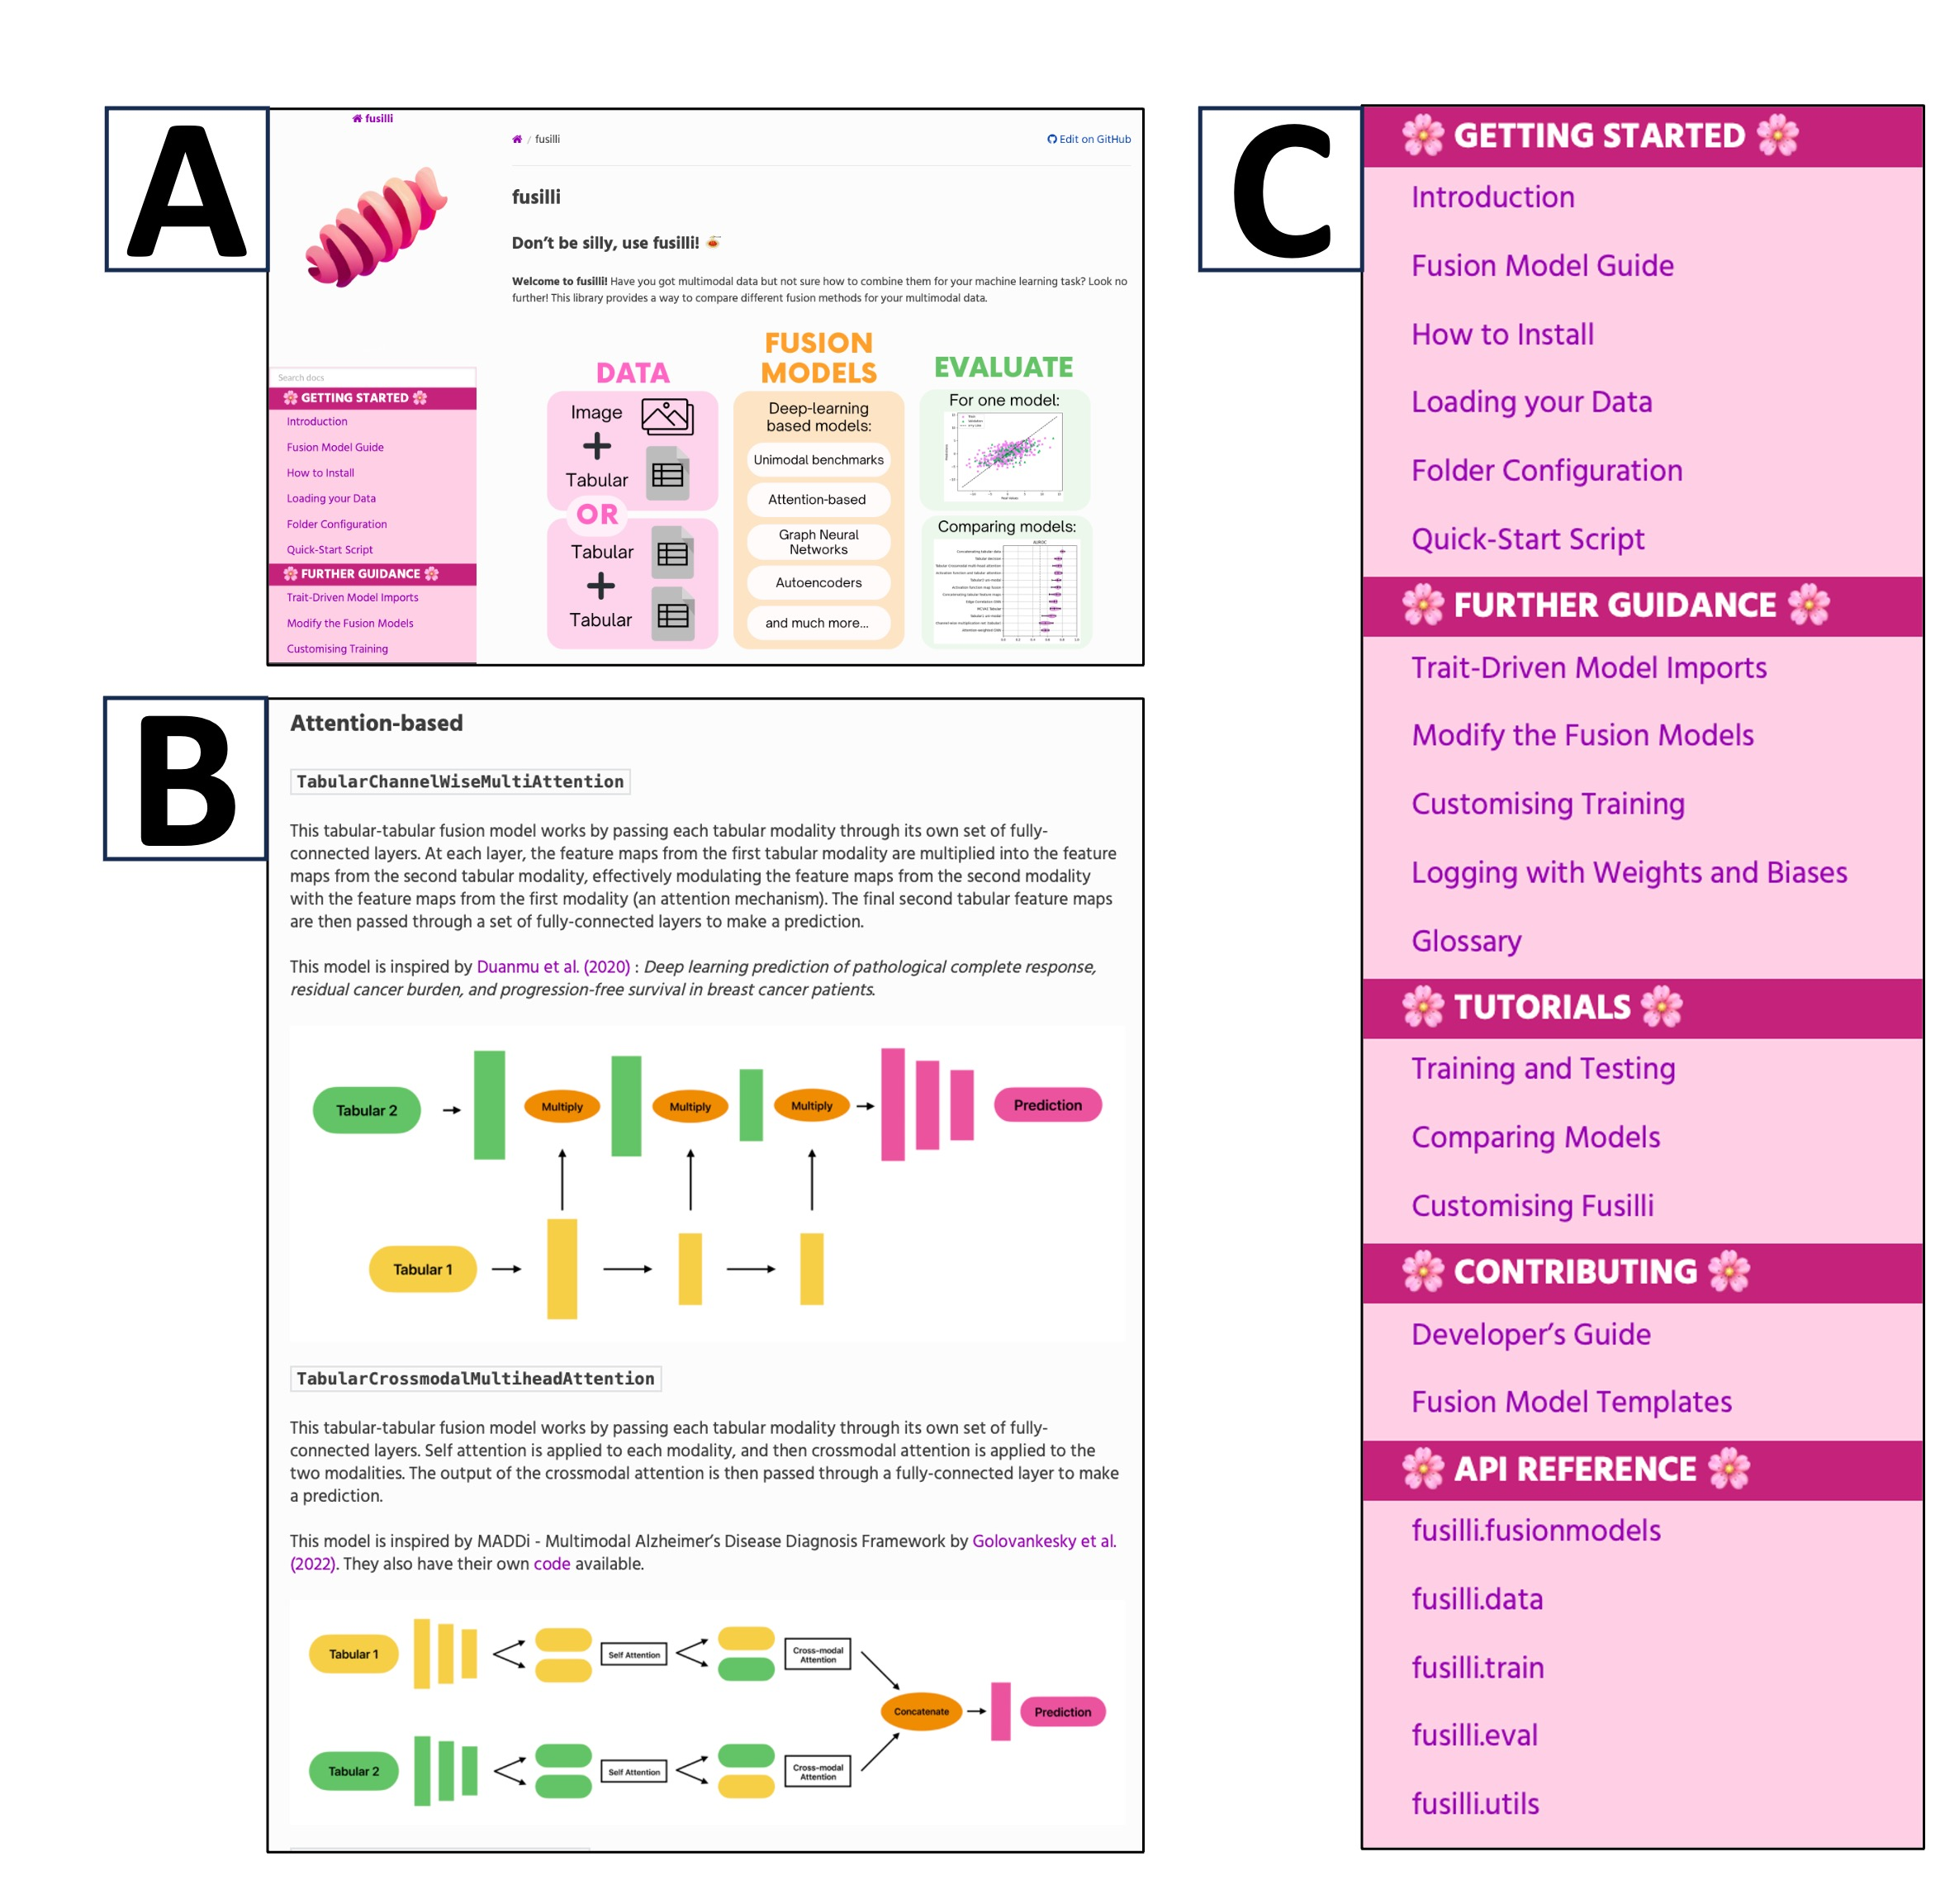
\includegraphics[width=1\linewidth]{figures/fusilli_documentation}
    \caption{Overview of the Fusilli documentation. \\
    \textbf{A}: The home page of the documentation, showing the logo and the diagram explaining Fusilli's purpose.\\
    \textbf{B}: Two examples of the fusion model explanations, complete with diagram and description with reference to source paper. \\
    \textbf{C}: The sidebar of the Fusilli documentation showing all the pages available.
    }
    \label{fig:fusillidocs}
\end{figure}

Figures~\ref{fig:fusillioutputs}A, B, and C show the figures output by Fusilli after training, validating, and comparing the models respectively.
The format of the figures depends on the prediction task and the type of training used, with the figures shown being for a binary classification task with 5-fold cross validation training.
If the user chooses to use train-test split training, the comparison figure is a bar chart instead of a violin plot.
Additionally, if the user trains a regression model, the performance evaluation will be a scatter plot of the predicted values against the true values.


\begin{figure}
    \centering
    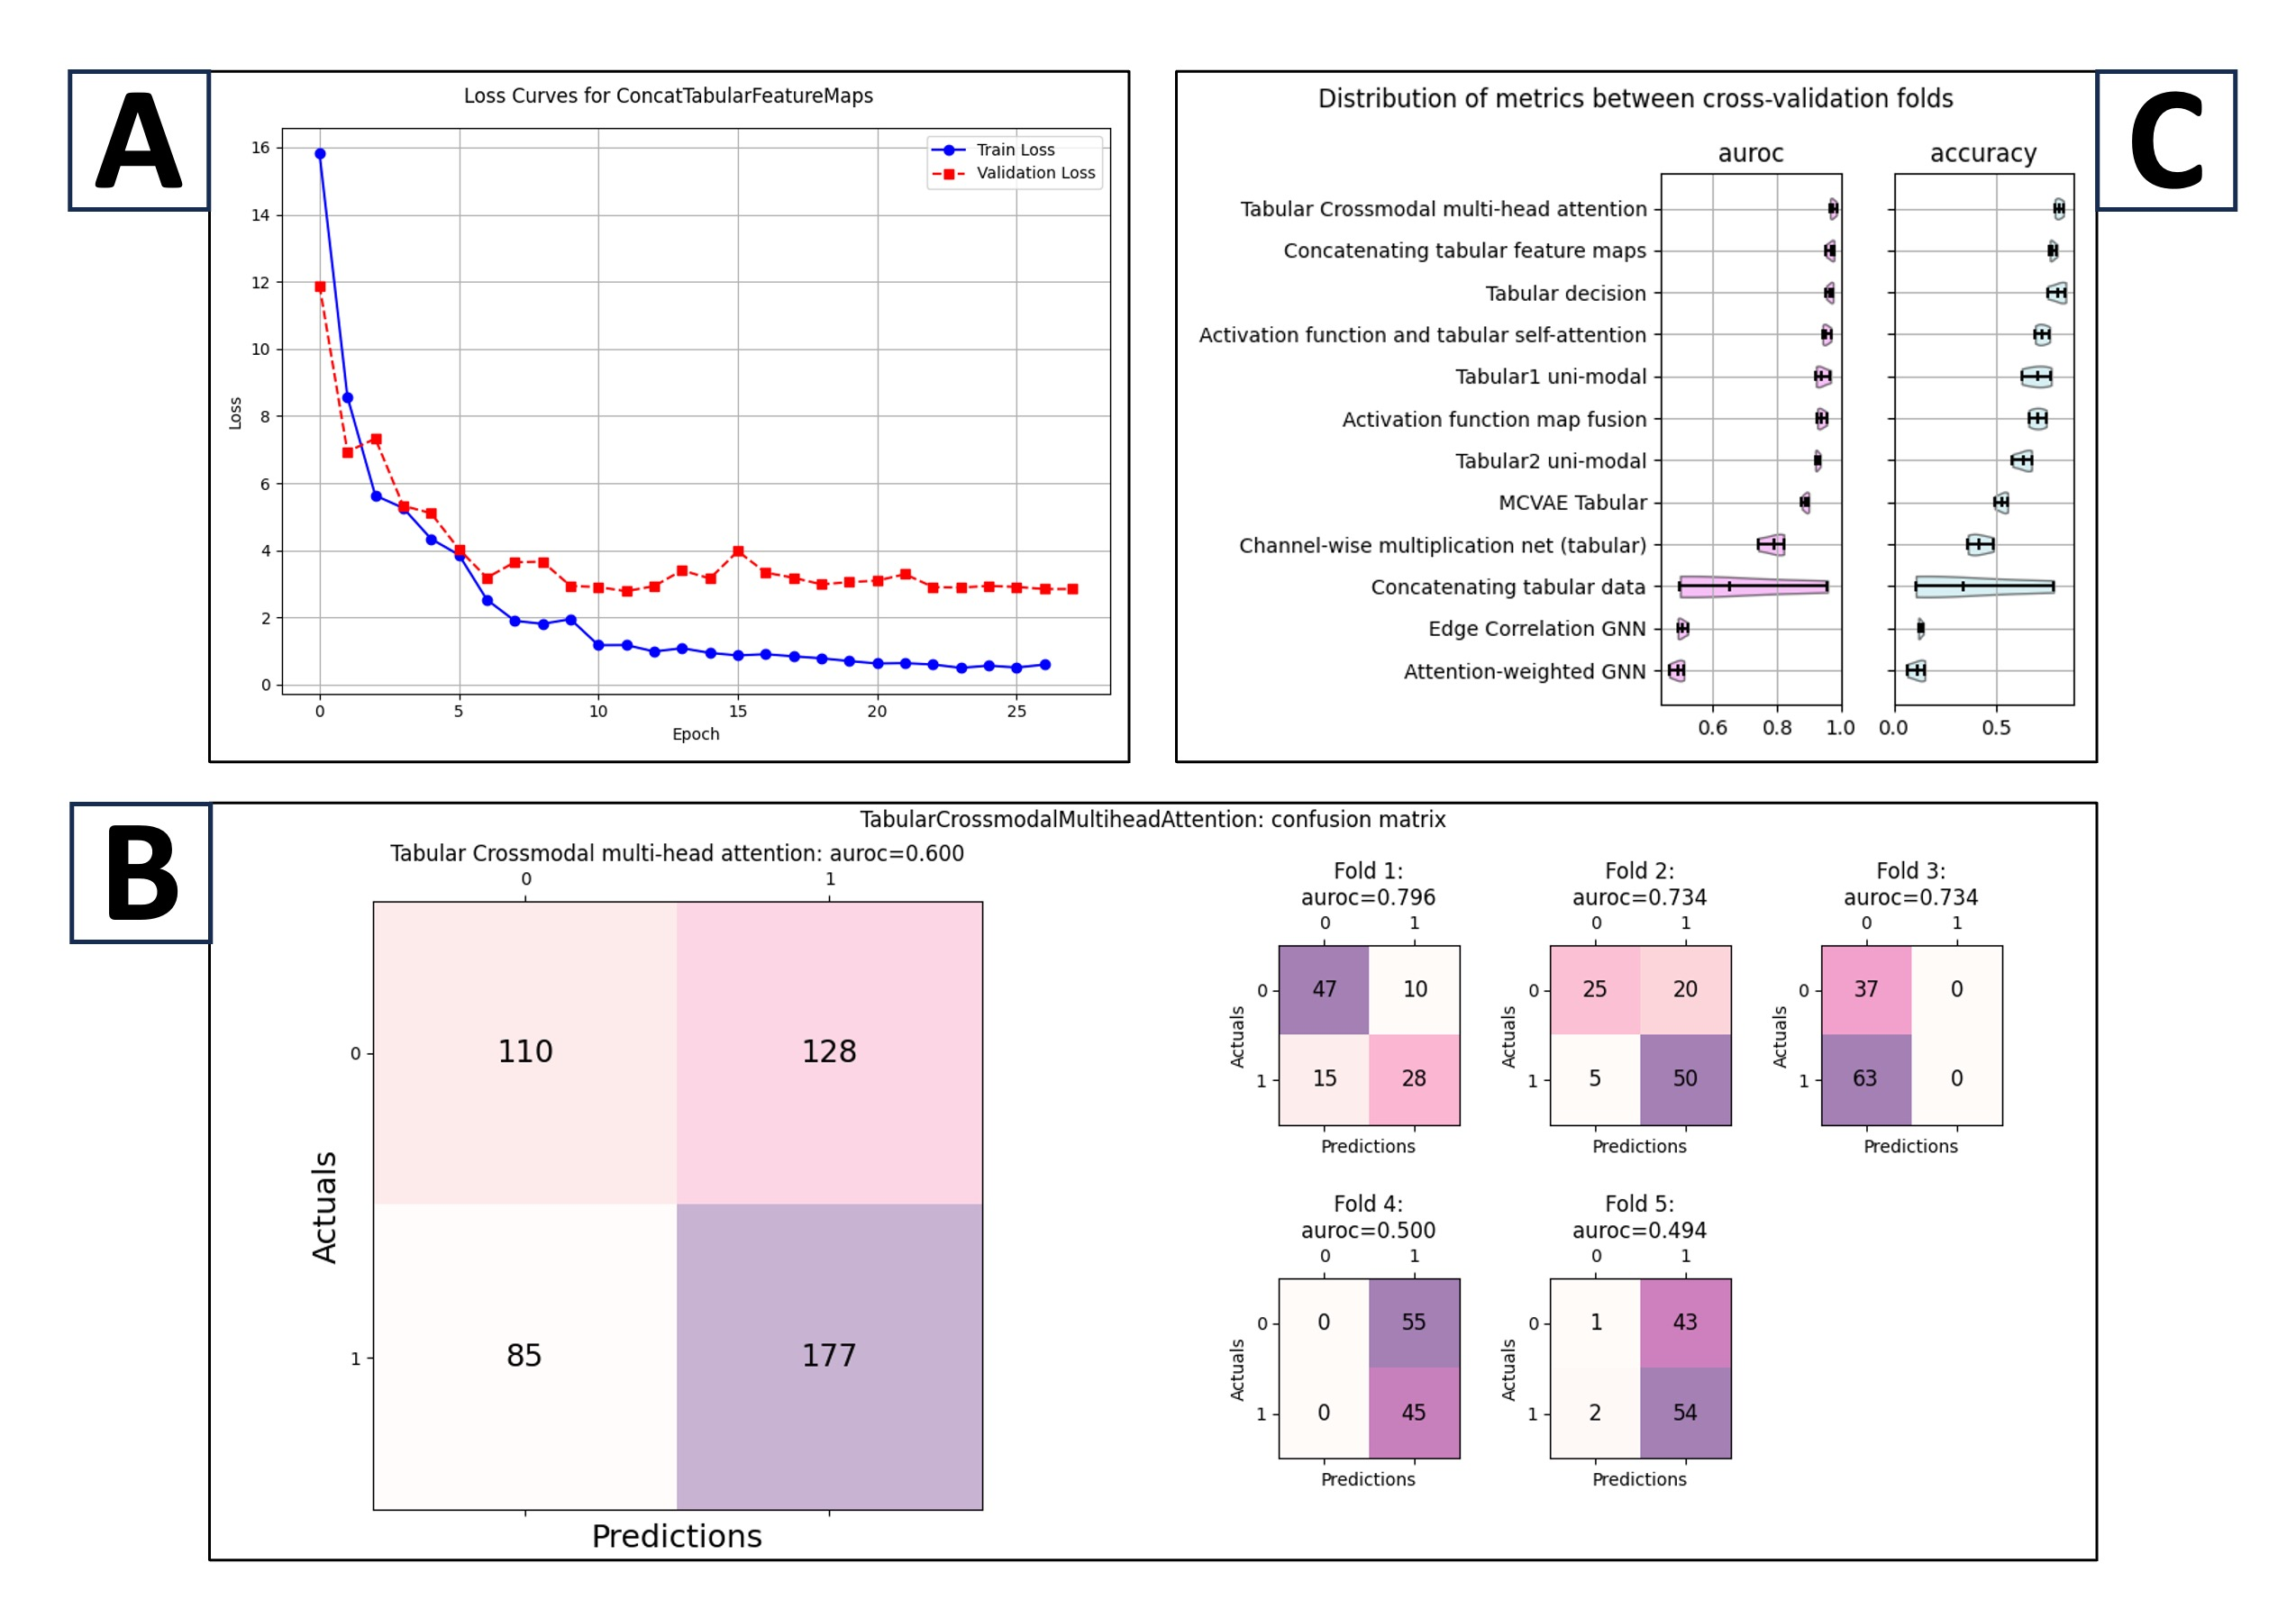
\includegraphics[width=1\linewidth]{figures/fusilli_outputs}
    \caption{Fusion model training, evaluation, and comparison figures output by Fusilli. \\
    \textbf{A}: The training and validation loss curves for an individual model.\\
    \textbf{B}: Performance evaluation of a model which was trained on a binary task with 5-fold cross validation. Both the validation performances of each fold and the overall performance from the aggregated folds are shown. \\
    \textbf{C}: Comparison of the models' performances on the validation data. The violin plot distributions are the distributions of the fold performances when using k-fold cross validation. If train-test split training is used, the comparison figure is a bar chart.
    }
    \label{fig:fusillioutputs}
\end{figure}


\section{Discussion}

Overall, Fusilli achieved the goals set out at the beginning of the project.
It has had interest from both beginners and experts, and there has been interest from people in different fields, such as thermal imaging.
Additionally, a hackathon project was run during the 2023 Centre for Medical Imaging Hackathon, where participants aimed to add new models to Fusilli, which was a success with two new models being added and more in development.

Fusilli has a number of limitations, most of which I hope to address with future updates to the software.
Firstly, Fusilli only supports two modalities, which is a limitation for tasks that may benefit from more than two modalities.
For example, in the context of MND prognosis prediction, using different types of MRI images (e.g. T1-weighted, T2-weighted, diffusion tensor imaging) could be beneficial, but Fusilli currently only supports one type of image alongside clinical information.
Moreover, Fusilli only supports inputting image data the form of PyTorch .pt files, which requires the user to do some pre-processing of their data.
This is a limitation for users who may not be comfortable with Python, and would prefer to input their data in the form of JPEGs or NiFTI files, for example.
Fusilli also only supports regression and classification tasks, and does not support other tasks such as time-to-event analysis.
Finally, although the models included in Fusilli are popular and cover a wide variety of architectures, there are many more models in the literature that could be included in Fusilli, and I hope to include these.

\section{Conclusion}
% Link to using fusilli on MND
In conclusion, Fusilli is a Python package for multimodal data fusion experimentation and analysis, specifically tackling the problem of lack of ways to compare models and lack of standardisation in the field.
I specifically made it for my PhD in fusing different data modalities in MND prognosis prediction.
The next chapter will discuss the application of Fusilli to MND prognosis prediction, using fusion of clinical information and brain region volumes.
% \begin{itemize}
%     \item Fusilli is a Python package for multimodal data fusion experimentation and analysis, specifically tackling the problem of lack of ways to compare models and lack of standardisation in the field.
%     \item I specifically made it for my PhD in fusing different data modalities in MND prognosis prediction
%     \item Link to next chapter on PPMI, ADNI, MIMIC: data fusion can be applied to any task where there are multiple data modalities describing one thing
%     \item Before going into MND, is there a clear benefit to different types of multimodal data fusion? Is there a consensus on the best approaches for different tasks?
%     \item MND sample size is small so we want to make sure we're using the best models by testing them on larger datasets with different applications
% \end{itemize}
